\documentclass[10pt]{article}
\usepackage[margin=0.82in]{geometry}
\usepackage[T1]{fontenc}
\usepackage{lmodern,microtype,amsmath,amssymb,booktabs,graphicx,xcolor}
\usepackage[colorlinks=true,urlcolor=teal,citecolor=teal,linkcolor=teal]{hyperref}
\usepackage{fancyhdr}
\pagestyle{fancy}\fancyhf{}\lhead{\small Known-prior calibration}\rhead{\small Independent research example}\cfoot{\thepage}
\setlength{\parindent}{0pt}\setlength{\parskip}{6pt}
\newcommand{\smallhead}[1]{\vspace{6pt}{\large\bfseries #1}\par}
\begin{document}
{\LARGE\bfseries Can a probability correction replace a coefficient refit?}\par
{\large A controlled comparison with optimization certificates and decision costs}\par
James N. Jean IV \hfill 28 October 2026\par
\textcolor{teal}{Independent portfolio research. GitHub research manuscript; not peer reviewed. Corrected retrospective evaluation (N1).}

\smallhead{The decision}
A score can become badly miscalibrated when positive events become rare. Refitting every feature coefficient is one response; shifting existing logits is another. This study asks when the cheaper structural change is a defensible starting point, while separating probability accuracy from the usefulness of the resulting alerts. It compares six prespecified methods on two exact public benchmark variants, with the target prevalence supplied as an experimental input.

At a supplied positive prevalence of 1\%, prior-odds correction substantially improves test log loss over unchanged scores. It does not consistently beat a fixed-penalty coefficient refit: it wins on one of five MAGIC splits and three of five MiniBooNE splits. Eight of ten conditional bootstrap intervals for that paired gap contain zero. Under the declared false-positive cost 10 and false-negative cost 1, the MAGIC adaptations flag no events at supplied prevalences up to 20\%. Better scores therefore do not establish a useful detector.

\smallhead{Why this comparison is useful}
The next step for a review-queue owner is to retain a simple prior correction as a measured baseline, verify that its assumptions fit the intended population, and evaluate the actual alert policy before replacing a model. This experiment establishes neither an unknown production prior nor a deployment recommendation. It does show a reproducible way to distinguish optimization success, predictive improvement and decision value.

The underlying correction is established, not novel. Saerens and colleagues describe adjustments to new class priors, including estimation of unknown priors \cite{saerens}. Here the prior is known by construction; their EM estimator is not reproduced. Alexandari and colleagues examine calibration in label-shift adaptation \cite{alexandari}. The contribution here is a bounded, fully retained comparison with independent convex-optimization and decision checks, rather than a new adaptation algorithm or evidence of a literature-wide research gap.

\smallhead{Exact sources and populations}
OpenML 44125 MAGIC Telescope v7 contains 13,376 rows; 115 exact full-row duplicates are removed before selecting 8,000 whole feature groups. Its 10 descriptors come from a Monte Carlo simulation. OpenML 44128 MiniBooNE v6 contains 72,998 rows; 171 exact duplicates are removed before selecting 8,000 whole groups with 50 supplied measurement descriptors. The original UCI sources credit R. Bock and Byron Roe respectively under CC BY4.0 \cite{magic,miniboone}. These OpenML variants have different counts and class balance from the original UCI files.

Selection follows sorted SHA256 feature signatures, capped at8,000 complete groups without target-dependent sampling. The selected positive counts are 4,041 and4,044. Each selected group has one row; no conflicting-label groups occur. Removing exact repeats changes empirical frequencies and does not prove the repeated events were errors. No acquisition/run identifiers are inferred, and no new physical measurements are collected.
\newpage

\smallhead{Protected fitting and controlled mixtures}
Five seeds 101, 202, 303, 404, 505 map whole feature signatures into disjoint fitting/validation/calibration/test partitions using a declared SHA256 modulo20 rule: 50/15/15/20\% by buckets. Every partition has at least 20 observations of each class. Splits overlap across seeds and are not independent replications. Feature means and population SDs are fitted only inside the corresponding fitting partition. Constant features receive scale 1.

For a target positive prevalence $q\in\{.01,.05,.20,.50\}$, assign positive rows weight $q/n_1$ and negative rows $(1-q)/n_0$. Weights sum to one and reproduce $q$ exactly. This changes the empirical class mixture while holding within-class values fixed. It is a controlled label-shift scenario, not a test of unknown-prior estimation, covariate shift or concept drift.

The base ridge-logistic objective is
\[
 L(\beta)=\sum_i w_i\{\log(1+\exp(z_i))-y_i z_i\}
       +\frac{\alpha}{2}\|\beta_{\rm feature}\|_2^2,\qquad
 z_i=x_i^\top\beta .
\]
The intercept is unpenalized. Choose $\alpha$ from
$\{10^{-4},10^{-3},10^{-2},.1,1,10\}$ using validation log loss, breaking ties toward smaller $\alpha$. Refit the selected base and scaler on fitting plus validation rows. Six of ten selected alphas lie at the grid's lower boundary; the finite search is not a regularization optimum.

\begin{center}\small
\begin{tabular}{p{.23\linewidth}p{.66\linewidth}}
\toprule
Method & Available information and fixed choice\\\midrule
Unchanged & Frozen base logit, without a target-prior adjustment.\\
Prior odds & Add $\operatorname{logit}(q)-\operatorname{logit}(\pi_{\rm base})$. Requires calibrated source probabilities and stable class-conditionals.\\
Intercept & Fit one additive offset on weighted calibration rows, restricted to $[-20,20]$.\\
Slope + intercept & Fit slope $[0,5]$ and offset $[-20,20]$ on the same weighted calibration rows.\\
Coefficient refit & Refit all coefficients on fitting+validation+calibration with$q$ weights, frozen selected$\alpha$ and frozen base scaler.\\
Known-prior constant & Predict $q$ for every event; checks whether scoring adds value beyond the supplied prior.\\
\bottomrule
\end{tabular}
\end{center}

All models and adaptations were frozen in Git commit
\texttt{155b69c0bea4fd815b34d23b745810d471f9ea43} before initial test scoring. Corrected fits were frozen at \texttt{49162586d96592f69b8787b241091c5df79a7048} before retrospective rescoring. The coefficient refit uses the same available labels as the base-plus-calibrator workflow but does not retune its penalty under $q$. It is not the best possible fully retuned system. Bounds are engineering choices, not empirically optimal values. No fitted slope or offset reaches a declared boundary.

\smallhead{Optimization evidence}
Ridge fits use two deterministic starts; slope/intercept fits use three.

L-BFGS-B uses declared \texttt{ftol}$10^{-14}$, \texttt{gtol}$10^{-9}$, maximum 5,000 iterations and maximum 50 line-search steps \cite{scipy}. Both ridge starts must succeed and agree in objective within absolute/relative $10^{-8}$. Intercept-only fits use a bracketed derivative root or the correct convex boundary.

The original L-BFGS-B-only run passed independent arithmetic and Windows replay but failed Linux coefficient equality. Correction N1 adds at most 20 Newton corrections on the same convex objectives, stopping at projected gradient $10^{-12}$, with bounded line search and retained trials. Independent final residual must be at most $10^{-11}$. No grid, split, prior, cost, bound or replay tolerance changed. All ten selected penalties and all decision losses remain unchanged. The original failure is preserved; this is a corrected retrospective evaluation of a previously inspected test.
\newpage

\smallhead{What the held-out scores say}
Primary scores are weighted log loss and Brier score, the probability MSE. At $q=1\%$, the medians below describe five overlapping splits per benchmark; they are not pooled population estimates.
\begin{center}\small
\setlength{\tabcolsep}{9pt}
\begin{tabular}{lrrrr}
\toprule
&\multicolumn{2}{c}{MAGIC simulation}&\multicolumn{2}{c}{MiniBooNE benchmark}\\
Method&Log loss&Brier MSE&Log loss&Brier MSE\\\midrule
Unchanged&0.524085&0.182740&0.269716&0.081670\\
Prior odds&0.047975&0.009690&0.034189&0.008582\\
Intercept&0.048006&0.009693&0.033928&0.008366\\
Slope + intercept&0.048007&0.009691&0.033107&0.008056\\
Coefficient refit&0.047615&0.009612&0.033274&0.008006\\
Known-prior constant&0.056002&0.009900&0.056002&0.009900\\\bottomrule
\end{tabular}
\end{center}
The paired median log-loss difference, prior odds minus coefficient refit, is $+0.000344$ nats for MAGIC and $-0.000421$ for MiniBooNE. These are medians of paired differences, not differences between separate medians. The sign changes across seeds. For the prespecified$q=.01$ comparison, 1,000 whole-group resamples per dataset/seed recompute class means and mix them at $q$. All 10,000 draws retain both classes; no invalid draw is silently replaced. Ordered groups, generator details, sample-index digests and every draw are retained.

\smallhead{Where score improvement fails to become decision value}
A hypothetical false-positive loss 10 and false-negative loss 1 imply an alert threshold $p\ge10/11$. The loss is $10FP+FN$ per weighted scenario event, not dollars or a measured detector cost. Flagging nothing has loss$q$. All four MAGIC adaptations issue no alerts across all five splits at $q\le.20$. Their score improvements do not produce a useful review queue under that threshold.

At $q=.05$ on MiniBooNE, prior odds has median decision loss $0.053404$, worse than the $0.05$ no-alert reference, and exceeds that reference in three of five splits. Intercept recalibration has median $0.043623$ but still exceeds the reference in two splits. The fixed-penalty refit has median $0.045590$ and also exceeds it in two splits. Choosing a method from these test decisions would reuse the test for selection; this report instead retains the declared comparison and identifies the need for a separate decision-validation design.

\smallhead{Independent checks and limits}
Every one of 340 optimization attempts passes successful-status, independently recomputed objective/gradient, directional finite-difference and Hessian checks. The largest independently recomputed final gradient or box-KKT residual is $9.06\times10^{-13}$, below $10^{-11}$; the smallest checked Hessian eigenvalue is $1.48\times10^{-4}$. The Hessian is a sum of nonnegative weighted outer products plus a nonnegative ridge term, hence positive semidefinite. Numerical certificates at tolerance are not exact-arithmetic proof or generalization guarantees.

Standard-library CSV/struct parsing independently reconciles all 86,374 source rows and every selected value against SciPy ingestion; SQLite checks group partitions and class counts. Independent scalar softplus and summation reconstruct 71,706 validation logits,386,112 test predictions,240 metric rows,48 displayed median cells and all 10,000 bootstrap draws. Eight adversarial contracts cover held-target isolation, prior weights, odds identity, extreme logits, gradients/KKT, failed-attempt rejection, Newton stationarity and invalid resampling draws.

Important limits remain: supplied priors and stable class-conditionals; only linear base models and a fixed penalty grid; unknown event/run dependence; source preprocessing and frequency changes; overlapping seeds; hypothetical costs; and no deployment, production-latency or financial-impact measurement.
\newpage

\smallhead{Reproduction and next study}
The public repository retains source metadata and hashes, bounded panels, the pre-test freeze, every numerical start and coefficient vector, observation-level predictions, all planned metrics and bootstrap draws, tests and executable checks:
\url{https://github.com/S3R3Bii/prior-shift-recalibration}.

The fresh-directory replay refits every model and adaptation, recomputes independent certificates and compares coefficients, all predictions, metrics, summaries and resamples at absolute $10^{-7}$/relative $10^{-9}$. Optimizer runtimes and iteration/evaluation counts remain evidence, not cross-machine equality targets. A clean exact-head Linux replay is a separate release gate; this manuscript does not replace that check.

A useful follow-up would estimate the target prior rather than supply it, then test calibration and alert policies on genuinely separate event runs with a justified cost and review budget. That experiment is not executed here. Neither a novel statistical method nor a literature-wide gap is claimed.

\begin{thebibliography}{9}\small
\bibitem{saerens} M. Saerens, P. Latinne and C. Decaestecker (2002). Adjusting the outputs of a classifier to new a priori probabilities: a simple procedure. \emph{Neural Computation} 14(1),21--41. \url{https://doi.org/10.1162/089976602753284446}.
\bibitem{alexandari} A. Alexandari, A. Kundaje and A. Shrikumar (2020). Maximum Likelihood with Bias-Corrected Calibration is Hard-To-Beat at Label Shift Adaptation. \emph{PMLR} 119,222--232. \url{https://proceedings.mlr.press/v119/alexandari20a.html}.
\bibitem{magic} R. Bock (2004). MAGIC Gamma Telescope. UCI Machine Learning Repository. DOI 10.24432/C52C8B. \url{https://archive.ics.uci.edu/dataset/159/magic+gamma+telescope}. CC BY4.0; exact OpenML 44125 v7 derivative used.
\bibitem{miniboone} B. Roe (2005). MiniBooNE particle identification. UCI Machine Learning Repository. DOI 10.24432/C5QC87. \url{https://archive.ics.uci.edu/dataset/199/miniboone+particle+identification}. CC BY4.0 attribution preserved; exact OpenML 44128 v6 derivative used.
\bibitem{scipy} SciPy 1.15.3 documentation. \texttt{minimize(method='L-BFGS-B')}. \url{https://docs.scipy.org/doc/scipy-1.15.3/reference/optimize.minimize-lbfgsb.html}.
\end{thebibliography}
\newpage
\smallhead{Probability performance at a rare-event prior}
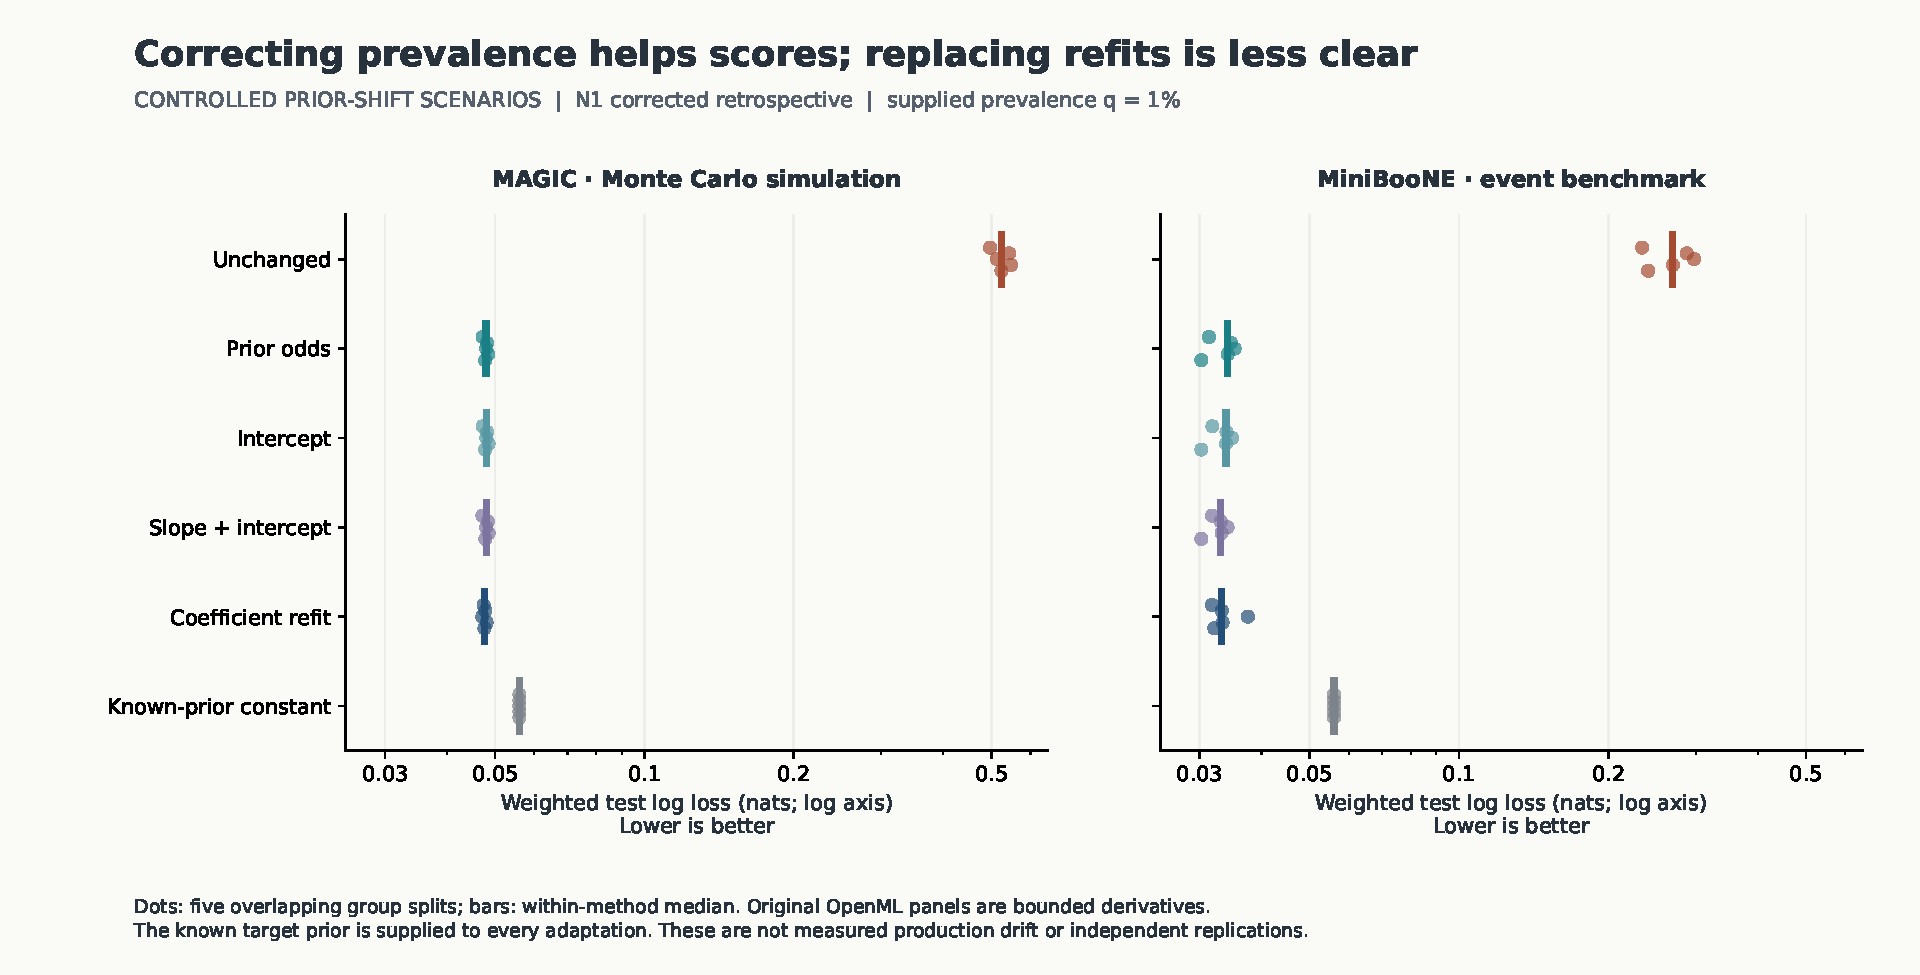
\includegraphics[width=\linewidth]{images/rare_probability_scores.pdf}
The supplied target prevalence is 1\%. The known-prior constant provides a stronger reference than raw accuracy. Score adaptation removes much of the mismatch from unchanged scores in these two variants. The fine differences among corrected methods require paired evaluation; this overview does not resolve a universal winner.
\newpage
\smallhead{Paired uncertainty, without pooling overlapping splits}
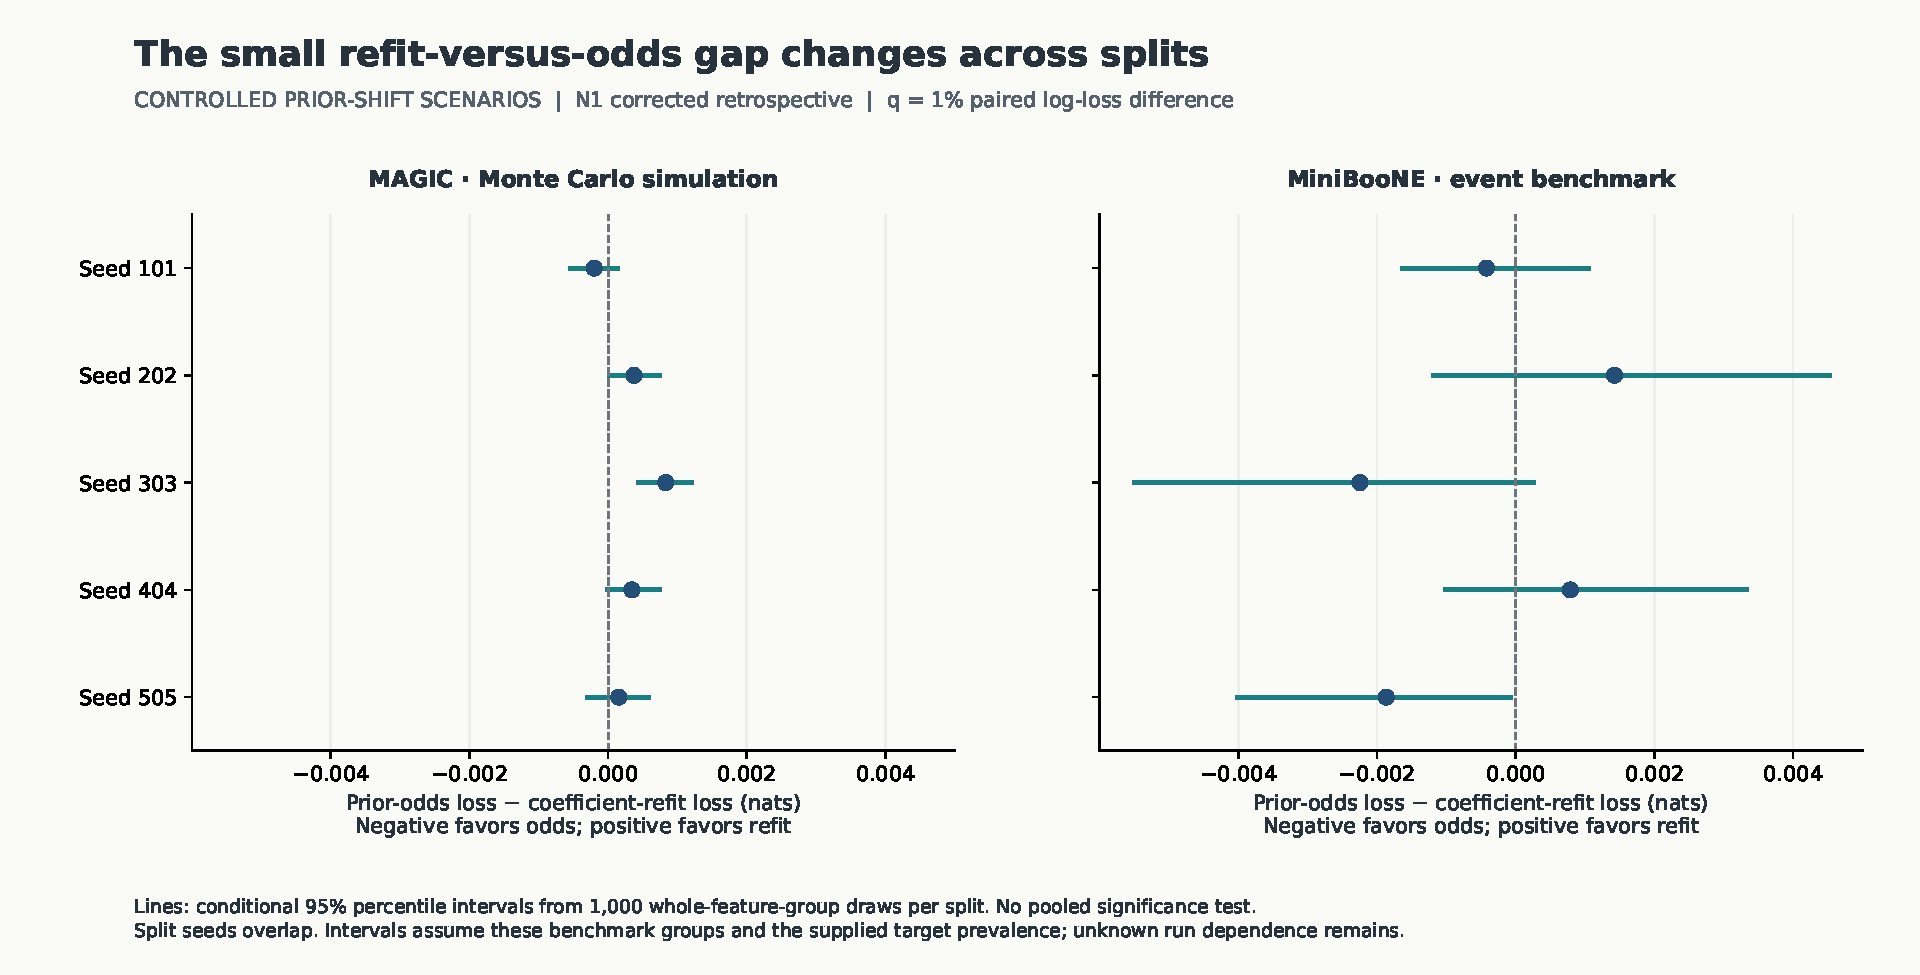
\includegraphics[width=\linewidth]{images/paired_refit_gap.pdf}
The intervals condition on whole feature groups and the scenario mixture. Eight of ten include zero, while one MAGIC interval favors the refit and one MiniBooNE interval favors odds correction. These overlapping-seed intervals are not ten independent confirmatory tests, and no multiple-comparison claim is made.
\newpage
\smallhead{The decision can disagree with the probability score}
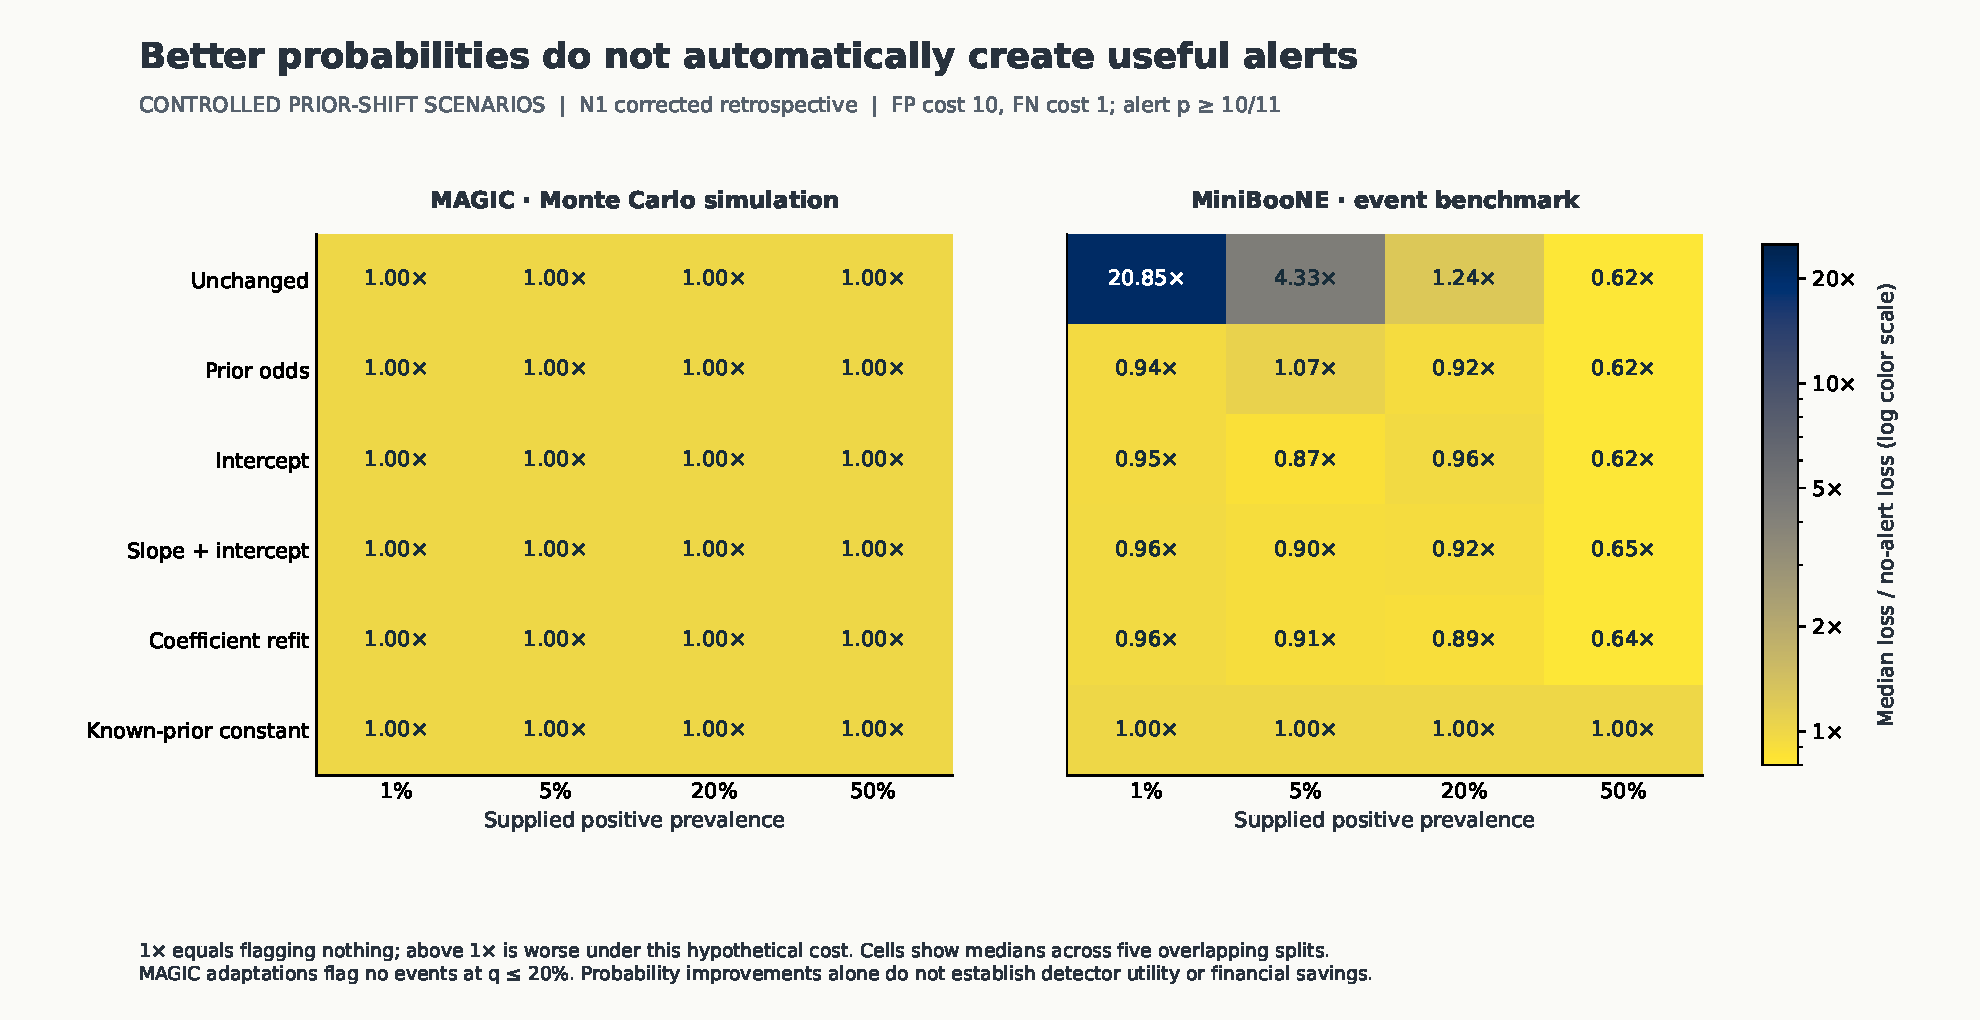
\includegraphics[width=\linewidth]{images/decision_loss_tradeoff.pdf}
The no-alert reference is exactly 1$\times$ in this display. Rounded MAGIC medians do not distinguish tiny changes near1; complete unrounded costs and confusion weights remain in the repository. MiniBooNE's unchanged score is especially costly in the 1\% scenario under the declared false-positive penalty. This is a hypothetical decision stress test, not a detector operating specification.
\end{document}